\normalfalse \difficilefalse \tdifficiletrue
\correctionfalse

%\UPSTIidClasse{11} % 11 sup, 12 spé
%\newcommand{\UPSTIidClasse}{12}

\exer{Système 4 barres $\star\star$ \label{C2:06:17}} 
\setcounter{question}{0}\UPSTIcompetence[2]{C2-06}
\index{Compétence C2-06}
\index{Système 4 barres}
\ifcorrection
\else
\marginnote{\textbf{Pas de corrigé pour cet exercice.}}
\fi

\ifprof
\else
On a : 
%\begin{multicols}{2}
\begin{itemize}
\item $\vect{OA} = a \vx{1}-f \vy{1}$ avec $a=\SI{355}{mm}$ et $f=\SI{13}{mm}$;
\item $\vect{AB} = b \vx{2}$ avec $b=\SI{280}{mm}$;
\item $\vect{BC} = -c \vx{3}$ avec $c=\SI{280}{mm}$;
\item $\vect{OC} = -d \vx{0}-e\vy{0}$ avec $d=\SI{89,5}{mm}$ et $e=\SI{160}{mm}$;
\end{itemize}
%\end{multicols}
%a,b,c,d,e,ff = 355,280,280,89.5,160,13

\begin{center}
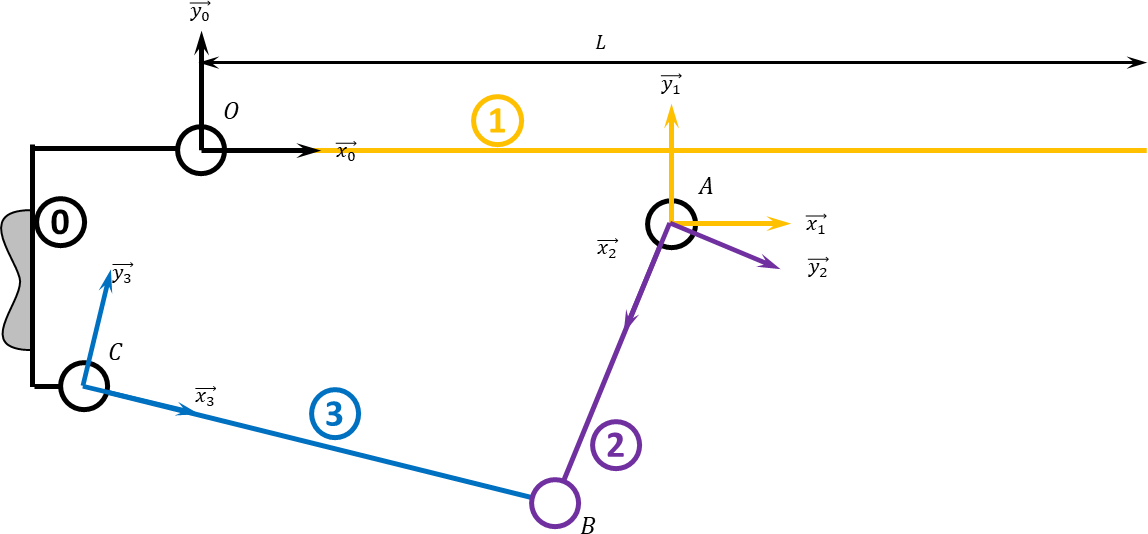
\includegraphics[width=\linewidth]{17_01}

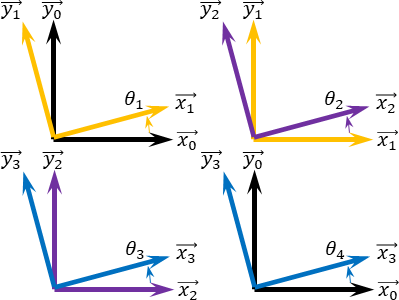
\includegraphics[width=\linewidth]{17_02}
\end{center}
\fi

\question{Tracer le graphe des liaisons.}
\ifprof
\else
\fi

\question{Exprimer $ \theta_1(t)$ en fonction de $\theta_4(t)$.}
\ifprof
\else
\fi

\question{Exprimer $\dot{\theta_1}(t)$ en fonction de $\dot{\theta_4}(t)$.}
\ifprof
\else
\fi

\question{En utilisant Python, tracer $\dot{\theta_1}(t)$ en fonction de $\dot{\theta_4}(t)$. On considérera que la fréquence de rotation de la pièce \textbf{1} est de 10 tours par minute.}
\ifprof
\else
\fi



\ifprof
\else
\begin{flushright}
\footnotesize{Corrigé  voir \ref{C2:06:17}.}
\end{flushright}%
\fi